\documentclass[12pt]{article}
\usepackage[spanish]{babel}
\usepackage[utf8x]{inputenc}
\usepackage{fancyhdr}
\usepackage[shortlabels]{enumitem}
\usepackage{setspace}
\usepackage[hidelinks]{hyperref}
\usepackage{graphicx}
\usepackage{natbib}
\usepackage{listings}
\usepackage{float, tikz,geometry,graphicx}
\usepackage{tabularx, enumitem}
\usepackage{listings}
\usepackage[T1]{fontenc}
\usepackage{beramono}
\usepackage{natbib}
\usepackage{longtable}
\usepackage{multirow}

\setcounter{tocdepth}{2} % Show sections

\definecolor{codegreen}{rgb}{0,0.6,0}
\definecolor{codegray}{rgb}{0.5,0.5,0.5}
\definecolor{codepurple}{rgb}{0.58,0,0.82}
\definecolor{backcolour}{rgb}{0.95,0.95,0.92}

\lstdefinestyle{c-style}{
    language=[GNU]C++,
    backgroundcolor=\color{backcolour},   
    commentstyle=\color{codepurple},
    keywordstyle=\color{orange},
    numberstyle=\tiny\color{codegray},
    stringstyle=\color{codegreen},
    basicstyle=\ttfamily\footnotesize,
    breakatwhitespace=false,         
    breaklines=true,                 
    captionpos=b,                    
    keepspaces=true,                 
    numbers=left,                    
    numbersep=5pt,                  
    showspaces=false,                
    showstringspaces=false,
    showtabs=false,                  
    tabsize=2
}

\author{Anthony Aguilar \and Christian Ledgard \and Alexander Baldeon}
\title{Proyecto - Teoría de la Computación}

% encabezados
\lhead[]{CS2101- UTEC \\Teoría de la Computación}
\chead[]{2020-1}
\rhead[]{Prof. Juan Gutierrez Alva \\jgutierreza@utec.edu.pe}
\renewcommand{\headrulewidth}{0.5pt}

% pie de pagina
\rfoot[]{}
\renewcommand{\footrulewidth}{0pt}
\renewcommand{\labelenumii}{\theenumii}
\renewcommand{\theenumii}{\theenumi.\arabic{enumii}.}

\pagestyle{fancy}



\begin{document}
  \begin{titlepage}
    \centering
    {\bfseries\LARGE Universidad de Ingeniería y Tecnología\par}
    \vspace{2cm}
    {\scshape\Large Ciencia de la Computación\par}
    \vspace{3cm}
    {\scshape\Huge Natural Language Processing with Context Free Grammar\par}
    \vspace{3cm}
    {\itshape\Large Proyecto - Teoría de la Computación\par}
    \vfill
    {\Large Autores: \par}
    {\Large Christian Ledgard Ferrero\par}
    {\Large Anthony Aguilar\par}
    {\Large Alexander Baldeon\par}
    \vfill
    {\Large Mayo 2020 \par}
  \end{titlepage}
  \thispagestyle{fancy}

\tableofcontents
\newpage

\section{Introducción}
 Hoy en día la tecnología está presente en muchos ámbitos de nuestra sociedad. Desde vehículos que se manejan por sí solos hasta en nuestros celulares que nos permiten estar más comunicados que nunca. Unos de los avances más significativos en los últimos tiempos son los asistentes virtuales como Siri, Alexa, Google Assistant, entre otros. ¿Alguna vez se han preguntado cómo estos sistemas organizan y analizan nuestras oraciones para ponerlas en un determinado contexto? Una posible implementación es utilizar \textbf{gramáticas independientes del contexto} para organizar y luego generar un árbol de \textit{"parseo"} con la oración. Esto se logra al tener un léxico y una gramática previamente definida.

\section{Alcance}
En nuestro proyecto nosotros realizaremos una investigación aplicada en donde desarrollaremos un algoritmo simple para realizar un parser  de acuerdo a un léxico y gramática previamente definida. Utilizaremos diversas fuentes \cite{box_2018}, \cite{L5CFG_2017}, \cite{NLPOverview}, \cite{CFGandParsing_2015}, \cite{CFGWiki}, \cite{CYKAlgorithmWiki}, \cite{EPWiki}, \cite{LRParser} y \cite{LLParser}. 

\section{Definición del Problema}
Cómo dividir una oración, utilizando gramáticas independientes del contexto, para que el computador pueda interpretarlas correctamente. ¿Casos de ambigüedad? ¿Qué hacer en determinados casos?


\section{Estado del Arte}
El inicio del procesamiento de lenguaje natural suele remontarse a 1950 cuando Alan Turing publicó el articulo 'Computing Machinery and Intelligence' donde propone lo que conocemos como el test de Turing, un criterio de inteligencia.
\\
Una de las primeras aplicaciónes del NLP ocurrió en 1954 e involucro la traducción de 60 oraciones rusas al inglés.
\\
En los 1960´s ELIZA y SHRDLU fueron sistemas capaces de comunicarce con  humanos.
\\
Existen al menos 4 algoritmos de parsing:
\begin{enumerate}
    \item El algoritmo CYK (Cocke–Younger–Kasami)
    \begin{enumerate}
        \item Solo trabaja con CFG en la forma normal de chumsky
        \item El peor de los casos es $O(n^3 . |G|)$ time. Donde $n$ es el tamaño de la cadena y $|G|$ es el tamaño de la gramática $G$ lo que lo hace uno de los mas eficientes en el peor de los casos.
    \end{enumerate}
    \item Earley parser
    \begin{enumerate}
        \item Trabaja con todas las gramáticas libres del contexto.
        \item Tiene un tiempo de ejecución $O(n^3)$ en el caso promedio,$O(n^2)$ en gramáticas no ambiguas y $O(n)$ para CFG deterministas.
    \end{enumerate}
    \item LR parser (Left-to-right, Rightmost derivation in reverse)\\
    Son tipos de bottom-up parsers que analizan DCFG en tiempo lineal.
    \begin{enumerate}
        \item LALR parser
        \item Canonical LR parser
        \item Minimal LR parser 
        \item GLR parser
    \end{enumerate}
    
    \item LL parser (Left-to-right, Leftmost derivation)\\
    Es un top-down parser para un subset de CFG
\end{enumerate}

\section{Propuestas}
\begin{itemize}
    \item Implementar y analizar un algoritmos de parseo para construir una gramática independiente del contexto bajo una gramática y un lenguaje dado.
    \item Analizar posibles implementaciones y soluciones en casos de ambigüedad y presentar propuestas utilizadas actualmente por grandes empresas como Amazon o Google.
\end{itemize}
\newpage

\section{Implementación de Algoritmos}

Para implementar los algoritmos CYK y Earley definimos primero que es una gramática.

\subsection{Clase Gramática}
Para la implementación de la estructura regla, la dividimos en 2 partes: Derecha e Izquierda. Ejemplo: izq -> der. La parte izquierda estará definida por un string y la derecha por un vector de strings. Asimismo, creamos la clase gramática que almacenará en un vector de punteros a reglas, todas las reglas a analizar.

\lstinputlisting[style=c-style]{codigo/gramatica.h}
%\lstinputlisting[style=c-style]{codigo/gramatica.cpp}

\newpage


\subsection{Algoritmo CYK}
El siguiente algoritmo, considerado 'bottom-up parsing', fue inventado por John Cocke, Daniel Younger y Tadao Kasami. Este solo opera con gramáticas en la forma normal de Chomsky \cite{CYKAlgorithmWiki}. 

Utilizando la notación Big O, el peor caso del algoritmo CYK es  
 ${\displaystyle {\mathcal {O}}\left(n^{3}\cdot \left|G\right|\right)}$ donde ${\displaystyle n}$ es la longitud de la cadena y ${\displaystyle \left|G\right|}$ es el tamaño de la gramática \cite{HopcroftUllman}. Esta complejidad hace que sea uno de los algoritmos más eficientes de parseo en términos del peor caso.

Cumpliendo con los estándares, utilizaremos programación dinámica para resolver el Algoritmo CYK. Conforme al pseudocódigo expuesto en la Figura \ref{fig:pCYK}, realizaremos la implementación en C++, orientada a objetos.

\begin{figure}[h!]
    \centering
    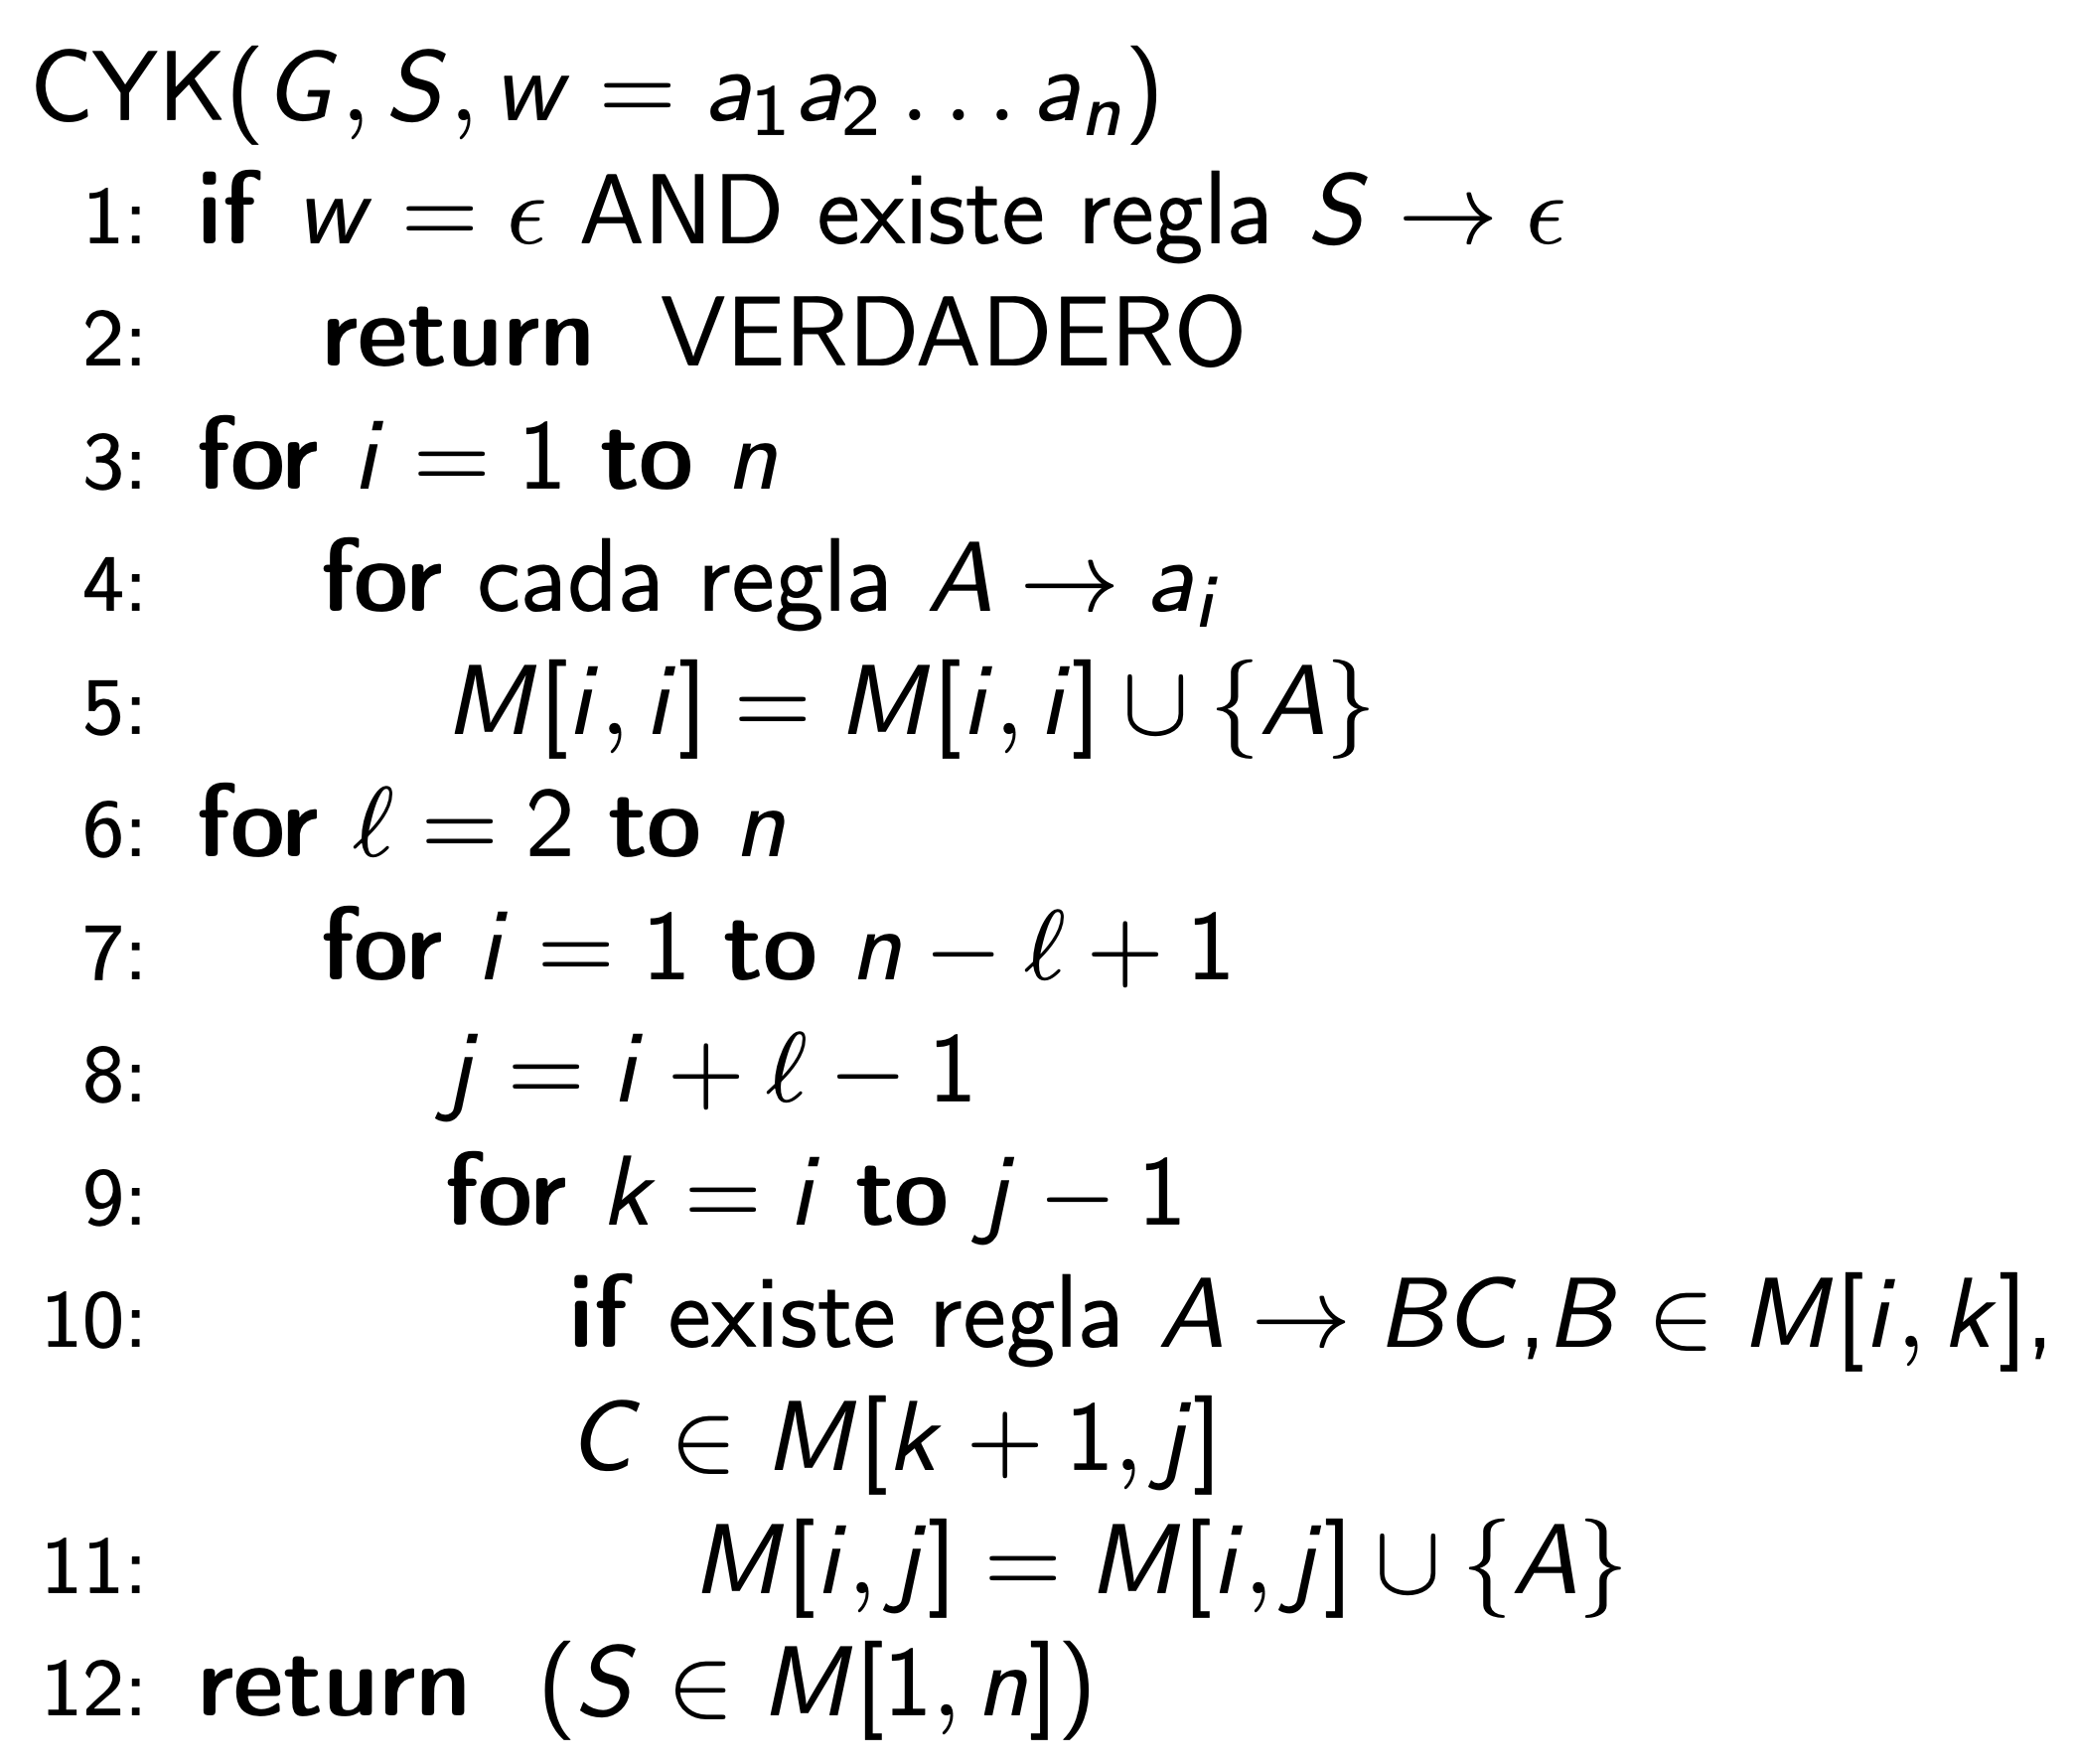
\includegraphics[width=250px]{img/pCYK.png}
    \caption{Pseudocódigo del algoritmo CYK}
    \label{fig:pCYK}
\end{figure} 

Nosotros creamos un array llamado matriz para almacenar el resultado ya procesado. Asimismo, en el método 'solve', ejecutaremos el algoritmo. Dicho método retornará un doble puntero, al puntero del array donde estará guardado nuestro resultado dinámico con la solución. También, en el método 'cadenaAceptada()', retornamos TRUE si la cadena es aceptada por el algoritmo, de lo contrario, retornaremos FALSE.

\lstinputlisting[style=c-style]{codigo/CYK.h}
%\lstinputlisting[style=c-style]{codigo/CYK.cpp}

\newpage


\subsection{Algoritmo Earley Parser}
A diferencia del algoritmo CYK el algoritmo de Earley es del tipo 'top-down' ya que éste evalúa si la cadena pertenece a la gramática empezando por la regla inicial y derivándola hasta obtener la cadena en el caso que ésta exista en la gramática.
\\\\
Para los siguientes párrafos $\alpha$, $\beta$ y $\gamma$ representan cualquier cadena de variables y símbolos de la gramática. $X$ y $Y$ representan variables de la gramática.Y $a$ representa cualquier símbolo de la gramática.
\\\\
Para lograr esta derivación se introduce una notación llamada 'dot-notation' o notación-punto $X \rightarrow \alpha \cdot \beta$. Esta notación indica que parte de una regla de la gramática ya ha sido reconocida (la parte a la izquiera del punto) y qué variable o símbolo se espera a continuación (la parte a la derecha del punto).
\\\\
Dada una cadena de tamaño $n$ se construye un array de tamaño $n+1$ donde cada posición en el array a partir de la posición 1 corresponde a un símbolo en la cadena correspondiendo la posición 0 al $\epsilon$ que precede a la cadena. Cada lugar en el array le corresponde a un conjunto de estados donde cada estado es una tupla que se construye a partir de una 'dot-notation' y la posición en el array donde 
ésta se originó $(X \rightarrow \alpha \cdot \beta, i)$. Llamamos al conjunto de estados que se encuentran en la posición $k$ $E(k)$.
\\\\

Este algoritmo consiste en repetir tres operaciones basadas en estos estados: predecir, escanear y  completar.

\begin{itemize}
    \item Predecir: para todos los estados en $E(k)$ de la forma $(X \rightarrow \alpha \cdot Y \beta,i)$, agregamos $(Y \rightarrow \cdot \gamma , k)$ a $E(k)$ para todas las producciones de la forma $Y \rightarrow \gamma$ en la gramática.
    \item Escanear: si $a$ es el siguiente símbolo a leer entonces para todos los estados en $E(k)$ de la forma $(X \rightarrow \alpha \cdot a \beta,i)$, agregamos $(X \rightarrow \alpha a \cdot \beta,i)$ a $E(k+1)$.
    \item Completar:  para todos los estados en $E(k)$ de la forma $(Y \rightarrow \gamma \cdot, i)$, buscamos todos los estados en $E(i)$ de la forma $(X \rightarrow \alpha \cdot Y \beta,j)$ y agregamos $(X \rightarrow \alpha Y \cdot \beta,j)$ a $E(k)$.
\end{itemize}

Notese que el tamaño de $E(k)$ puede aumentar de tamaño después de cada operación así que se tiene que realizar las respectivas operaciones a los nuevos estados generados por operaciones previas.

\lstinputlisting[style=c-style]{codigo/Earley.h}
%\lstinputlisting[style=c-style]{codigo/Earley.cpp}


\newpage

\bibliography{bibliografia}  
\bibliographystyle{ieeetr}

\end{document}
